%%%%%%%%%%%%%%%%%%%%%%%%%%%%%%%%%%%%%%%%%%%%%%%%%%%%%%%%%%%%%%%%%%%%%%%%%%
%%%%%%%%%%%%%%%%%%%%%%%%%%%%%%%%%%%%%%%%%%%%%%%%%%%%%%%%%%%%%%%%%%%%%%%%%%
\section*{CHEMISCHE BINDUNG}
%%%%%%%%%%%%%%%%%%%%%%%%%%%%%%%%%%%%%%%%%%%%%%%%%%%%%%%%%%%%%%%%%%%%%%%%%%
%%%%%%%%%%%%%%%%%%%%%%%%%%%%%%%%%%%%%%%%%%%%%%%%%%%%%%%%%%%%%%%%%%%%%%%%%%

%%%%%%%%%%%%%%%%%%%%%%%%%%%%%%%%%%%%%
	\begin{karte}{
		Wie ist die generelle Beziehung zwischen der Gr��e eines Atoms und seiner ersten Ionisierungsenergie?
		 Welches Element hat die gr��te Ionisierungsenergie? Welches die kleinste?
		}
		\begin{enumerate}
		\item
		Je gr�{\ss}er das Atom desto kleiner seine Ionisierungsenergie. \\
		
		Ionisierungsenergie ist die Energie, die ben�tigt wird, um ein Atom oder Molek�l zu ionisieren,  d. h. um ein Elektron vom Atom oder Molek�l zu trennen. 
		Allgemein ist die n-te Ionisierungsenergie die Energie, die ben�tigt wird, um das n-te Elektron zu entfernen. \\
		d.h.: Die Ionisierungsenergie nimmt im Allgemeinen von links nach rechts zu und nimmt von oben nach unten ab. \\
		
		kleinste: \ce{He} \\
		gr�{\ss}te: \ce{Fr}

	\end{enumerate}
		
	\end{karte}
%%%%%%%%%%%%%%%%%%%%%%%%%%%%%%%%%%%%%


%%%%%%%%%%%%%%%%%%%%%%%%%%%%%%%%%%%%%
	\begin{karte}{
		Identifizieren Sie das Element, dessen Ionen die folgende Elektronenkonfiguration haben: \\
			a) ein 2+Ion mit $[\ce{Ar}]3d^{9}$, \\
			b) ein 1+Ion mit $[\ce{Xe}]4f^{14}5d^{10}6s^{2}$.\\
			c) Wie viele freie Elektronen besitzen die Ionen?
		}
		\begin{enumerate}
	
			\item
			$[\ce{Ar}]3d^{9} + 2e^{-} 				\longrightarrow [\ce{Ar}]3d^{10}4s^{1}				=\ce{Cu}$
			
			\item
			$[\ce{Xe}]4f^{14}5d^{10}6s^{2} + e^{-} 	\longrightarrow [\ce{Xe}]4f^{14}5d^{10}6s^{2}6p^{1}		=\ce{Tl}$
			
			\item
			\textcolor{red}{hm? }
			
	
		\end{enumerate}
	\end{karte}
%%%%%%%%%%%%%%%%%%%%%%%%%%%%%%%%%%%%%


%%%%%%%%%%%%%%%%%%%%%%%%%%%%%%%%%%%%%
	\begin{karte}{
		Warum ist Kalzium im Allgemeinen reaktiver als Magnesium? Warum ist Kalzium im Allgemeinen weniger reaktiv als Kalium?
		}
		Je gr�{\ss}er das Atom desto kleiner seine Ionisierungsenergie. \\
		Die Ionisierungsenergie nimmt im Allgemeinen von links nach rechts zu und nimmt von oben nach unten ab
	\end{karte}
%%%%%%%%%%%%%%%%%%%%%%%%%%%%%%%%%%%%%


%%%%%%%%%%%%%%%%%%%%%%%%%%%%%%%%%%%%%
	\begin{karte}{
		Orden sie die folgenden Elemente nach ihrem Schmelzpunkt: $K,Br_{2},Mg,O_{2}$.
		Erkl�ren sie die Faktoren, die die Reihenfolge bestimmen.
		}
		\begin{enumerate}
		
				\item
				\ce{O2}(-218�C) < \ce{Br2}(-7�C) < \ce{K}(63.3�C) < \ce{Mg}(639�C)
				
				\item
				Bei der Metallenbindung(Elektronengas) nimmt die Anziehung zwischen Elektronengas und Atomkernen 
				mit der Anzahl der Au�enelektronen zu also \ce{Mg} > \ce{K}
				
				\item
				
		
			\end{enumerate}
	\end{karte}
%%%%%%%%%%%%%%%%%%%%%%%%%%%%%%%%%%%%%


%%%%%%%%%%%%%%%%%%%%%%%%%%%%%%%%%%%%%
	\begin{karte}{
		Phosgen hat folgende Elementzusammensetzung: 12,14\% \ce{C}, 16,17\% \ce{O} und 71,69\% \ce{Cl} (Massenprozent) 
			und ein Molekulargewicht von $98.9\: g/Mol$.\\
			Bestimmen sie die Molek�lformel dieser Verbindung. \\
			Zeichnen sie die Lewis- Strukturformel dieser Verbindung und argumentieren Sie warum
			Sie eine Bestimmte (von mehreren m�glichen) ausgew�hlt haben.
		}
		\begin{enumerate}
		
				\item
				$M_{\ce{C}}	=12\frac{g}{Mol}$\\
				$M_{\ce{O}}	=16\frac{g}{Mol}$\\
				$M_{\ce{Cl}}	=35,5\frac{g}{Mol}$\\
				$\Rightarrow \ce{COCl2}$
				
				\item
				Man w�hlt die Lewis-Strukturformel, in der die Formalladungen der Atome am N�chsten bei Null sind.\\
				Man w�hlt die Lewis Strukturformel, in der sich die negativen Ladungen an den elektronegativeren Atomen befinden.\\
				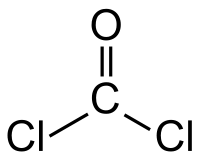
\includegraphics[width=0.15\textwidth]{_images/Phosgen.png}
		
		
			\end{enumerate}
	\end{karte}
%%%%%%%%%%%%%%%%%%%%%%%%%%%%%%%%%%%%%


%%%%%%%%%%%%%%%%%%%%%%%%%%%%%%%%%%%%%
	\begin{karte}{
		Ein unbekannter Stoff liefert eine Elementaranalyse von: \ce{C}: 68.13\%,
			\ce{H}: 13.72\%, \ce{O}: 18.15\% (Massenprozent). \\
			Bestimmen sie die Molek�lformel dieser Verbindung. \\
			Zeichnen sie mindestens drei reale Molek�le, die der Molek�lformel entsprechen.
		}
		
		\begin{enumerate}
		
				\item 
				$M_{\ce{C}}	=12\frac{g}{Mol}$\\
				$M_{\ce{H}}	=1\frac{g}{Mol}$\\
				$M_{\ce{O}}	=16\frac{g}{Mol}$\\ 
				
				$\ce{C}:	\frac{68,13}{12}		=5,72Mol\%$\\
				$\ce{H}:	\frac{13,72}{1}		=13,72Mol\%$\\
				$\ce{O}:	\frac{18,15}{16}		=1,13Mol\%$\\ 
				
				$5,72 : 13,72 : 1,13 \Rightarrow 5:12:1 \Rightarrow \ce{C5H12O}$
				
				\item
		
			\begin{minipage}{0.2\textwidth}%
				\centering
				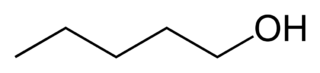
\includegraphics[width=\textwidth]{_images/Pentanol}%
			\end{minipage}%
			\hspace{1cm}
			\begin{minipage}{0.2\textwidth}%
				\centering
				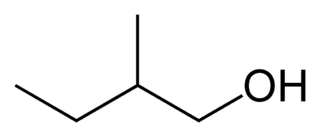
\includegraphics[width=\textwidth]{_images/2-Methyl-1-butanol}
			\end{minipage}%
			\hspace{1cm}
			\begin{minipage}{0.2\textwidth}%
				\centering
				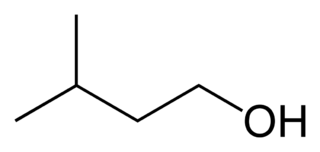
\includegraphics[width=\textwidth]{_images/3-Methyl-1-butanol}%
			\end{minipage}%
				
				
			\end{enumerate}
		
	\end{karte}
%%%%%%%%%%%%%%%%%%%%%%%%%%%%%%%%%%%%%


%%%%%%%%%%%%%%%%%%%%%%%%%%%%%%%%%%%%%
	\begin{karte}{
		Beschreiben Sie anhand einer Skizze s�mtliche Bindungen in Ethylen mit Hilfe des Konzepts der Hybridisierung. Bezeichnen Sie die Orbitale die Sie zeichnen.
		}
		
		\begin{enumerate}
			
				\item 
				Eine sigma-bindung ist eine einfachbindung zwischen zwei Atomen. 
				
				hier im ethen w�ren das die bindungen zu den wasserstoffatomen 
				und eine bindung zwischen den kohlenstoffatomen. 
				
				die $\pi$-bindung ist bei doppel- und dreifachbindungen vorhanden. zus�tzlich zur einen $\sigma$-bindung. 
				
				bei der $\pi$-bindung �berlappen zwei p-orbitale, also nicht hybridisierte...  
				
				da im ethen ja nur eine doppelbindung vorhanden ist, brauchst du also nur ein nichthybridisiertes p-orbital pro 
				Kohlenstoffatom. 
				also k�nnen die zwei anderen p-orbitale mit dem s orbital hybridisieren und man erh�lt: 
				sp2 davon h�tten wir ja dann drei st�ck pro C-Atom. 
				
				und das passt ja dann auch: zwei bindungen zu wasserstoffatomen und eine bindung zum anderen kohlenstoffatom. 
				und die zwei p-orbitale �berlappen einander und bilden zweite bindung, die doppelbindung
		
				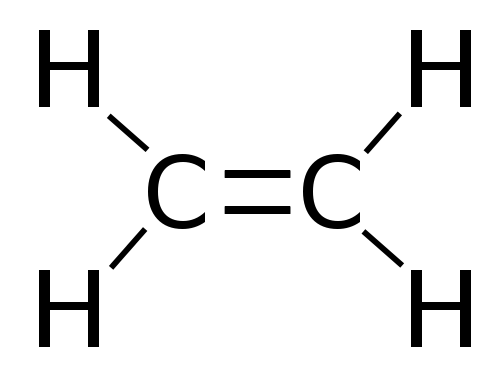
\includegraphics[width=0.2\textwidth]{_images/Ethen.png}	% angle width height scale
			
			\end{enumerate}
		
	\end{karte}
%%%%%%%%%%%%%%%%%%%%%%%%%%%%%%%%%%%%%


%%%%%%%%%%%%%%%%%%%%%%%%%%%%%%%%%%%%%
	\begin{karte}{
		Zeichnen sie das Molek�lorbitalschema f�r \ce{O2}.
		}
		
		\begin{enumerate}
			\item 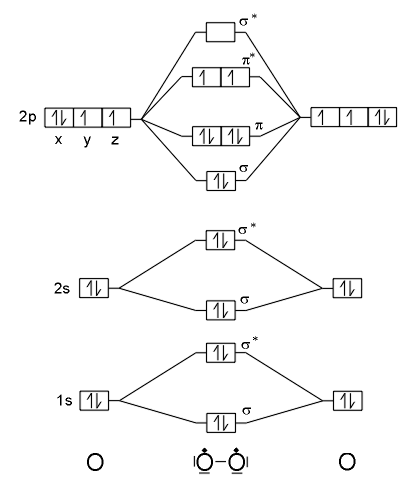
\includegraphics[width=0.5\textwidth]{_images/sauermo.png}
			
			\end{enumerate}
		
	\end{karte}
%%%%%%%%%%%%%%%%%%%%%%%%%%%%%%%%%%%%%


%%%%%%%%%%%%%%%%%%%%%%%%%%%%%%%%%%%%%
	\begin{karte}{
		Eine Verbindung, die aus 2.1\% \ce{H}, 29.8\% \ce{N} und 68,1\% \ce{O} besteht, hat
			ein Molekulargewicht von ca. 50 g/Mol. \\
			Wie lautet die Molek�lformel der Verbindung? \\
			Zeichnen sie die Lewis-Formel, wenn \ce{H} an \ce{O} gebunden ist. \\
			Wie ist die Struktur des Molek�ls? \\
			Wie ist die Hybridisierung der Orbitale am \ce{N}-Atom? \\
			Wie viele $\sigma$ - und $\pi$ -Bindungen gibt es in dem Molek�l?
		}
		
		\begin{enumerate}
			
				\item 
				$M_{\ce{H}}	=1\frac{g}{Mol}$\\
				$M_{\ce{N}}	=14\frac{g}{Mol}$\\
				$M_{\ce{O}}	=16\frac{g}{Mol}$\\ 
				
				$\ce{H}:	\frac{2,1}{1}		=2,1Mol\%$\\
				$\ce{N}:	\frac{29,8}{14}		=2,13Mol\%$\\
				$\ce{O}:	\frac{68,1}{16}		=4,26Mol\%$\\ 
				
				$2,1 : 2,13 : 4,26 \Rightarrow 1:1:2 \Rightarrow \ce{HNO2}$
				
				\item
				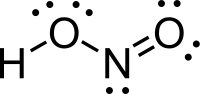
\includegraphics[width=0.2\textwidth]{_images/Lewis_Formel_Salpetrige_Saeure.png}
				
				\item
				Die Struktur ist trigonal eben.
				
				\item
				sp$^{2}$-Hybridisierung um N
				
				\item
				3 $\sigma$-Bindungen und 1 $\pi$-Bindung
				
			
			\end{enumerate}
		
	\end{karte}
%%%%%%%%%%%%%%%%%%%%%%%%%%%%%%%%%%%%%



